\documentclass[11pt]{article}
\usepackage{graphicx, float}
\parindent=0in
\parskip=8pt
\begin{document}
\title{COMP 512 - Project Report - Part 2}
\author{Luke Emery-Fertitta - Student ID: 260569374 \\ Jonathan Campbell - Student ID: 260481285}
\date{2015 November 11}
\maketitle

\section*{System Architecture}

The lock manager is stored at the middleware server. It receives lock requests from the transaction manager, which specifies the lock type (read or write), the data item to lock, and the ID of the transaction requesting the lock. It uses this centralized model so that the resource managers themselves need know nothing about locking. This approach also simplifies the process of waiting on a lock, since the middleware will know not to accept anymore operations from the same transaction until the lock is received (or a deadlock occurs), instead of having to be told by a resource manager who is waiting that it should wait as well. \par

The lock manager uses the strict 2PL locking scheme. Operations that read a data item will request a shared lock on the item. More than one transaction can receive a shared lock for the same data item. Operations that write a data item will request an exclusive lock on the item, which will only be given if there are no shared locks on that item, except for its own. If the transaction does have a shared lock and requests an exclusive lock, the lock is converted to exclusive if possible. If other transactions already have a shared lock on that item, then the requesting transaction will wait until those are released. Transactions will release all their locks only at commit or abort time. \par

The transaction manager is also contained entirely on the middleware server. Again, this design greatly simplifies the message passing requirements. Because the lock manager is local, the only message passing required after a request is received is the data access, which was already implemented in the first part of the project. Upon server initialization, a transaction manager is created. Then, we simply pass off the \texttt{start}, \texttt{abort}, and \texttt{commit} methods from the API directly to the transaction manager. \par

The \texttt{start} method initializes a transaction and provides the client with a transaction identifier to use with all other operations. This method atomically grabs the next available, unique transaction identifier integer, creates a \texttt{Transaction} object, and begins the TTL timer for the transaction. \par

When an operation is sent from the client to the middleware to be performed, the middleware will ask the transaction manager for the necessary locks and also inform it of the operations to perform in case of an abort (the undo operations). These operations are exactly the reverse of the operation sent by the client, e.g., if the operation was removeFlight, the undo operation will be addFlight, with the necessary parameters. The undo operation is passed as a Runnable using the lambda functionality in Java 8. After informing the TM of these details, the middleware will perform the requested operation, forwarding it to a resource manager if appropriate. When it receives the result of the operation, it will check if the operation succeeded or failed - in the latter case, it will ask the TM to remove the last undo operation, since there is nothing to undo. \par

The \texttt{abort} method is available as an API call. Additionally, aborts will automatically be performed upon deadlocks, as a form of deadlock resolution, and TTL expirations, as a form of client timeout handling. The TTL expiration is checked by a \texttt{ScheduledExecutorService}, which is simply a scheduled, concurrent operation that ensures the transaction has been used within a specified time period. In this case, ``used'' refers to any read or write operation which is called with the transaction identifier.  \par

When a transaction is aborted, the transaction manager will run the undo operations that have built up throughout the transaction's lifespan, ask the lock manager to release any locks held by the transaction, and remove the transaction from its transaction list. \par

When a transaction commits, the TM asks the LM to release the transaction's locks, and removes the transaction from its list. \par

The \texttt{shutdown} method is an API call for a full-system, soft shutdown. If the client requests a shutdown, the transaction manager will deny any future start transaction requests and wait for all running transactions to complete. After this, each of the resource managers is sent a shutdown request and the middleware terminates. The resource managers will exit gracefully upon receiving the shutdown message from the middleware. \par


\section*{Problems encountered}

One problem that was encountered that originated from the centralized model was the management of undo functions. Since the middleware contains the transaction manager, it is also responsible for informing the TM of the undo operations to perform in case of abort, before the actual operation takes place. Therefore, the middleware will need to know the reverse of each operation, even when it is only forwarding the operation to a resource manager. The undo operations are hardcoded in the middleware, so knowledge about each operation must reside at both middleware and RMs, which breaks the pattern of functional isolation. Further, some undo operations are more complex, in cases where an operation (like addFlight) can have different effects based on data state (it can add a completely new flight, or edit details of a current flight), leading to a necessity for state analysis on the middleware and communication with the RM to determine which action will be performed, in order to record the correct undo operation. \par

Concurrency was a concern due to the multithreaded request handling and asynchronus requirements of the transaction manager. We had to ensure that the transaction identifier was unique regardless of \texttt{start} execution order, and that once a shutdown request has been initiated, no client is able to start a new transaction. The former problem was solved with an \texttt{AtomicInteger} attribute, which allows for an atomic get and increment. The latter problem was solved by synchronizing the shutdown and start methods and adding an \texttt{isShutdown} attribute, such that once the shutdown has begun, threads will block at \texttt{start}, and after it finishes, transactions will fail to start. \par

\section*{Testing}

To test the lock manager, we created a framework to easily specify transactions and their specific operations to be executed. A Transaction Simulation class (TxnSimul) receives as input a series of integers representing the operations that the transaction should execute, with each group of four integers specifying the transaction ID, data item, lock type (read or write), and the amount of seconds to sleep after executing the operation. With this latter argument, it is possible to interleave the operations of two different transactions. The TxnSimul objects once created are inserted into an array, and then a new thread is created for each, so that all run concurrently. We created several tests in this format to verify the integrity of the lock manager, including the following schedules, with reasoning for each:

\begin{itemize}
\item T1 reads A, T1 writes A, T1 commit (lock conversion)
\item T1 reads A, T2 reads B, T2 writes A, T1 writes B, T1 commit, T2 commit (deadlock detection)
\item T1 reads A, T2 reads A, T2 commit, T1 writes A, T1 commit (check that read lock can be acquired on object with read lock already, and unlocking of locks upon commit)
\item T1 reads A, T2 reads A, T1 writes A, T1 commit, T2 commit (check if shared lock blocks other's write)
\end{itemize}

Specific particularities of scheduling prevented by two-phase locking such as dirty reads, writes, unrepeatable reads, etc., were not tested here since it was assumed that the provided 2PL locking implementation was sound. \par

With regards to testing of the transaction manager, sequences of commands were manually inputted into the client console with verification of results. Testing of undo operations was of particular focus, as well as concurrent modification situations (to verify correctness of locks).\par

\section*{Performance Analysis}

\subsection*{Technique}

For both parts, we use testing clients that repeatedly submit two transaction types. One is a middle-ware only transaction containing three customer read operations and three write operations. The other uses all three resource managers, performing a read and a write at each one. Each experiment can have the number of clients and delay between transactions varied, allowing us to controll transactions per second.

\subsection*{Results}

\begin{table}[H]
\centering
\caption{Performance of Single-Client Tran}
\begin{tabular}{c|c}
Type & Average Response Time(s) \\
\hline
Local MW & 0.0445 \\
Local RM & 0.1000 \\
Network MW & 0.0915 \\
Network RM & 0.1704 \\
\end{tabular}
\end{table}

\begin{figure}[H]
\centering
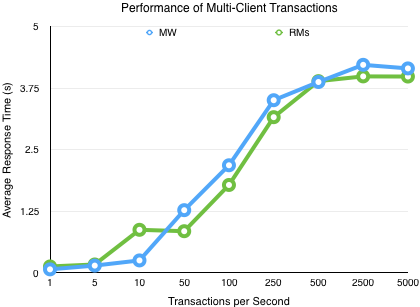
\includegraphics[scale=1]{plot.png}
\end{figure}

\subsection*{Analysis}

\textbf{Single-Client Observations:} \\
Network operations take roughly twice as long as local operations. RM transactions take roughly twice as long as their MW counterparts.\par

\textbf{Single-Client Analysis:} \\
There is network latency, and increased message hops for RM transactions. \par

\textbf{Multi-Client Observation:}\\
Initially, RM-only transactions have a longer average response time than MW-only transactions. This swaps near 40 tps. After that, both increase at steady exponential rate (due to the logarithmic $x$-axis scale) with MW-only transactions being a constant amount above RM. At 500 transactions per second these amounts converge, followed by a slight increase in the response time on the part of the middleware. Both converge and plateau at 5000 transactions per second. \par

\textbf{Multi-Client Analysis:}\\
Between 1 and 40 tps, the RM transactions take longer due to the message transfer overhead. This may be a bit extreme at 10 tps and could be slightly exaggerated by noise. After this, the limiting factor is the bottlenecking due to lock conflicts, which continues to become more severe. There may also be network congestion, contributing to the increase to a lesser degree. Finally, the plateau occurs due to the limitation on the Java client. We can only send so many transactions per second, so although we set the parameters for 10,000 tps, we are unable to actually achieve that number. Due to this insufficiency, we are capped in the number of transactions per second that can be tested.

\end{document}
